\section{Positive and Unlabeled Learning}
\label{sec:pulearning}

\noindent \textit{This part should explain the necessarity of Positive and Unlabeled Learning setup, including the importance to make a difference between inexaustive annot. and misclassification.}

\noindent
We discussed in Section \ref{sec:robustness} that misclassification and inexaustive annotation can have negative influence on feature transferability, which is undesirable when we train transferable weights with noisy data.
Therefore, methods to compensate these errors are discussed in this section.
In practice, misclassification error is less likely to \textit{dorminate} and dorminate means the misclassified rate outperforms the correct rate.
However, unannotated objects can be dorminant for a large dataset.
Besides,
the most studied \cite{reed2014training,sukhbaatar2014training,patrini2016making,jindal2016learning}
Therefore, we focus on inexaustive annotation.

%%%%%%%% TEXT PU Learning setup
\paragraph{Formulation}
\noindent \textit{This part should formulate the problem with a probability model and make clear statement that model here is different from previous section: model to corrupt and model to recover.}
\noindent
When we synthesized errors in Section \ref{sec:robustness}, we assumed that the observed labels depend on
$p(\tilde{y} \vert x, y)$.

$p(\tilde{y_{ij}} \vert y_{ij})$.
This model is easy to apply when we have the perfect annotations and want to generate noisy labels, but it is not as easy when we observe noisy labels and want to recover the correct ones.

$p(\tilde{y_{ij}} \vert y_{ij})$


%%%%%%%% TEXT Modeling
\paragraph{Weighted Logistic Regression}
\noindent \textit{This part should discuss the linear model for observing positive conditioning on true positive and its relationship to changing the class weight.}


%%%%%%%% TEXT Exponential loss
\paragraph{Exponential Loss for unlabeled examples}
\noindent
\textit{This part should explain why the exponential loss could perform better than the cross-entropy loss, potentially with a figure of 2D Gaussians.}
The ``soft'' bootstrapping loss in \cite{reed2014training} is actually equivalent to a softmax regression with \textit{minimum entropy regularization}\cite{grandvalet2005semi} which was originally proposed for semi-supervised learning.
Minimum entropy regularization encourages the model to have a high confidence in predicting labels.

%%%%%%%% TEXT Expontial loss FADE IN

\paragraph{Implementation details}
\noindent \textit{This paragraph should explain fade-in was introduced to avoid all-positive inital prediction;}

\noindent

%%%%%%%% TEXT Imbalanced
\noindent
\textit{This part should explain the influence of the imbalanced problem and how to overcome.}



%%%%%%%% FIGURE MOONS
\begin{figure*}
\begin{center}
% \fbox{\rule{0pt}{2in} \rule{.9\linewidth}{0pt}}
   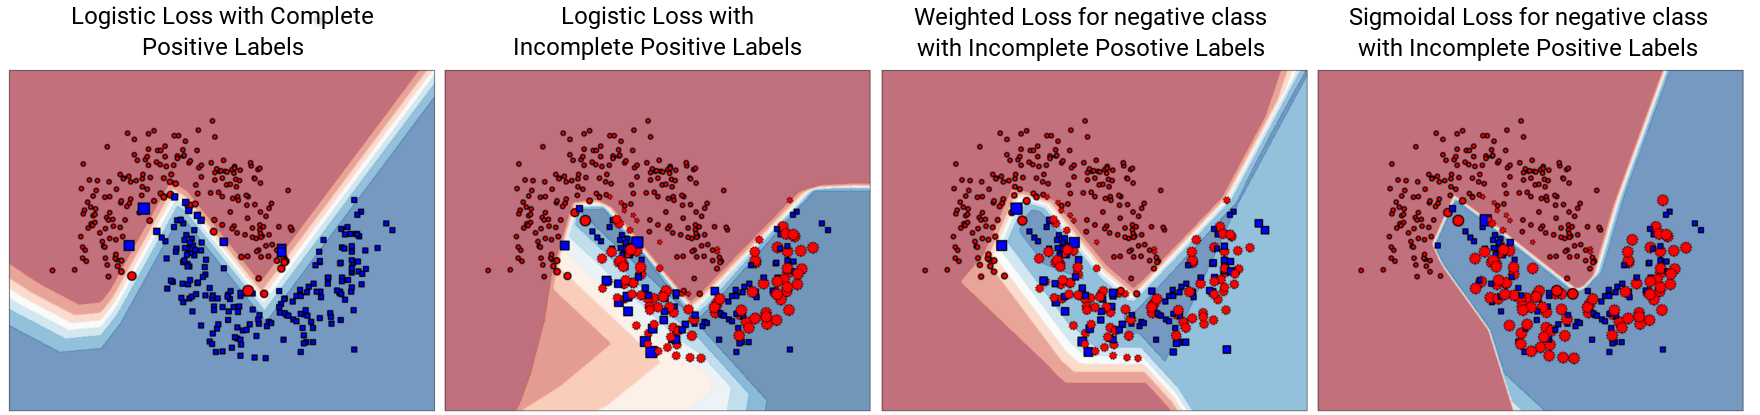
\includegraphics[width=0.95\linewidth]{img/moons.png}
\end{center}
   \caption{2D moons dataset with non-linear separable decision boudary. Four hundreds samples per class were drawn randomly from two interleaving half circles with noises added with a minor standard deviation. A \textbf{red circle} indicates an example labelled as positive whilst a \textbf{blue square} indicates the example has a negative label. The \textbf{leftmost} figures have complete positive labels, meaning the positive and negative labels are all correct, whereas, in \textbf{the other figures} only half of the positives were correctly labelled and the rest were mixed with the negative samples. The \textbf{background colors} represent the probability for the area to be positive given by the classifier trained with the given samples and labels: \textbf{red} for high probability areas, \textbf{blue} for low probability areas and \textbf{white} for the class transition areas, i.e.decision boundaries. The \textbf{size of the markers} in the top row denotes the per-class normalized training losses and the \textbf{size of the markers} in the bottom row the per-class normalized derivatives w.r.t the output of the last layer for the trained Multilayer Perceptron (MLP) with the different losses.}
\label{fig:moons}
\end{figure*}


%%%%%%%% FIGURE Losses
\begin{figure}[t]
\centering
% \fbox{\rule{0pt}{2in} \rule{0.9\linewidth}{0pt}}
   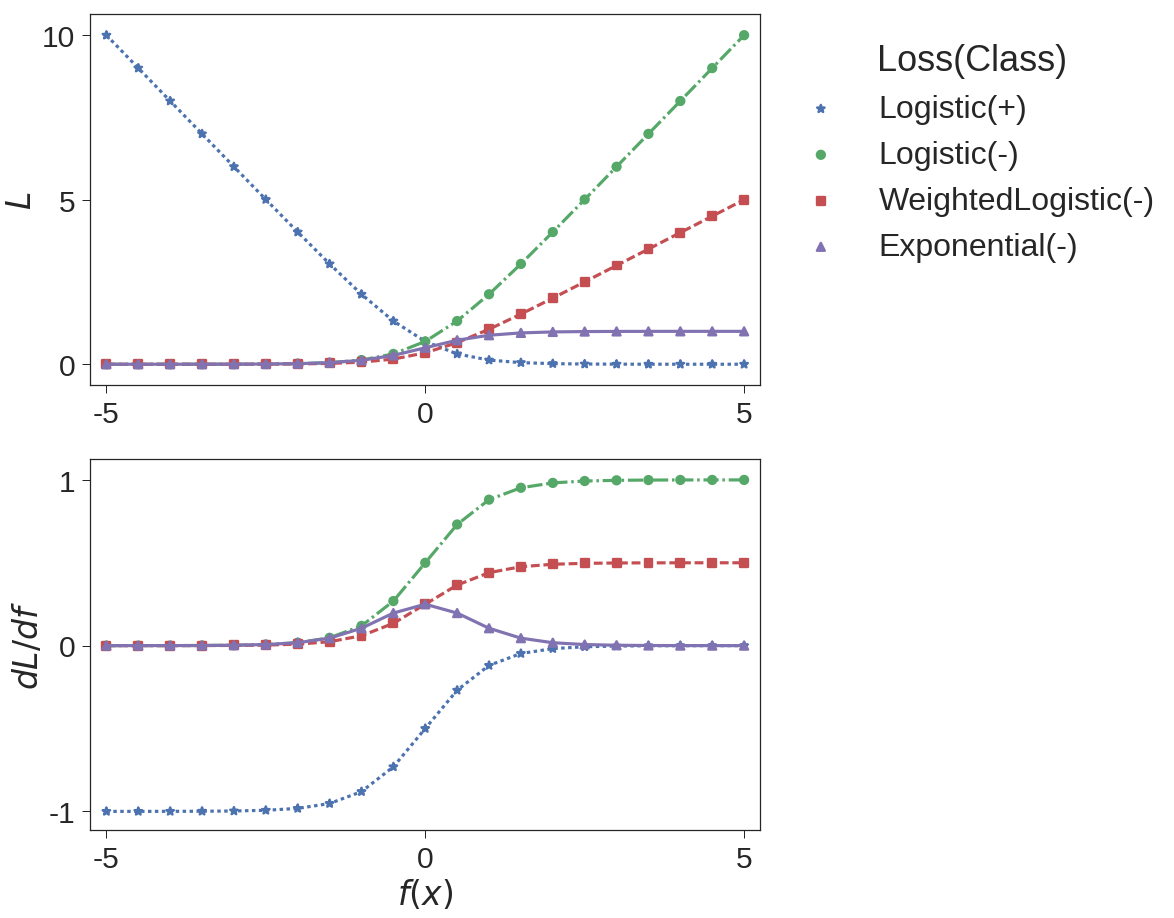
\includegraphics[width=0.95\linewidth]{img/losses.png}
\caption{The Logistic Loss, Weighted Logistic Loss, Exponential Loss and their dirivatives with respect to the model output.}
\label{fig:losses}
\end{figure}


%%%%%%%% FIGURE Varying positive annotating percetage
\begin{figure}[t]
\centering
\fbox{\rule{0pt}{2in} \rule{0.9\linewidth}{0pt}}
  %  \includegraphics[width=0.95\linewidth]{img/}
\caption{Varying percentage of annotated positives 10\%, 20\%, 50\%, 80\% and 100\% with images from CIFAR10 as the positives and images from CIFAR110 as the negatives.}
\label{fig:pct_annotating}
\end{figure}

%%%%%%%% TABLE CIFAR10
\begin{table}[t]
\resizebox{\columnwidth}{!}{
\centering
\begin{tabular}{ll|llll}
Annotation  & Loss & acc. & prec. & rec. & $F_1$ \\
\hline
Complete    & CrossEntropyU.   & $0.87\pm0.01$ & $0.88\pm0.01$ & $0.82\pm0.01$ & $0.85\pm0.01$ \\
50\%(P+N)   & CrossEntropyU.   & $0.83\pm0.01$ & $0.84\pm0.01$ & $0.78\pm0.01$ & $0.80\pm0.01$ \\
50\%P+U     & CrossEntropyU.   & $0.64\pm0.04$ & $0.93\pm0.08$ & $0.34\pm0.02$ & $0.44\pm0.06$ \\
50\%P+U     & WeightedU.       & $0.78\pm0.01$ & $0.75\pm0.01$ & $0.75\pm0.01$ & $0.76\pm0.01$ \\
50\%P+U     & ExponentialU.    & $0.82\pm0.01$ & $0.86\pm0.01$ & $0.73\pm0.01$ & $0.78\pm0.01$ \\
50\%P+U     & BootstrapHard    & $0.74$ & $0.81$ & $0.60$ & $0.67$ \\
50\%P+U     & DropoutReg.      & & & & \\
\end{tabular}
}
\caption{Image classification with positive examples partially annotated. The complete dataset contains images from CIFAR10 as the \textbf{positive} (P) set and images from CIFAR110 as the \textbf{negative} (N) set. The unannotated positive examples from P set construct the \textbf{unlabeled} (U) set together with the N set.}
\end{table}


%%%%%%%% TABLE
\begin{table}[t]
\resizebox{\columnwidth}{!}{
\centering
\begin{tabular}{ll|llll}
Annotation  & Loss & pixel acc. & mean acc. & mean IU & f.w. IU \\
\hline
Complete    & CrossEnt.U    &  &  & & \\
50\%(P+N)   & CrossEnt.U    & & & & \\
50\%P+U     & CrossEnt.U    & & & & \\
50\%P+U     & WeightedU        &  &  & & \\
50\%P+U     & ExponentialU     &  &  & & \\
50\%P+U     & BootstrapHard    &  &  & & \\
50\%P+U     & DropoutReg. & & & & \\
\end{tabular}
}
\caption{Image semantic segmentation with images contain single instance only from the PASCAL VOC2011 segmentation dataset. The complete \textbf{positive} (P) set denotes the foreground instances and the \textbf{negative} (N) set consists of the background. The unannotated instances from P set construct the \textbf{unlabeled} (U) set together with the N set.}
\end{table}
